% diffuse/intro.tex          pdflatex ZhCvGo15

% Predrag                               24jul2016
% Predrag                                3dec2015
% Tingnan                                2nov2015
% Predrag initial draft                 21nov2014
%         extracted from ChaosBook.org
% \Chapter{diffusion}{2apr2014}{Deterministic diffusion}

% \section{Introduction}

The advances in the theory of dynamical systems have brought a new
life to Boltzmann's mechanical formulation of statistical mechanics,
especially for systems near or far from equilibrium, and yielded new
sets of microscopic dynamics formulas for macroscopic observables such
as the transport coefficients. Sinai, Ruelle and Bowen (SRB) have
generalized Boltzmann's notion of ergodicity for a constant energy
surface of a Hamiltonian system in equilibrium to {nonequilibrium} steady states
of dissipative systems\rf{sinai,Rue76,bowen}. In this
more general setting the attractor plays the role of a constant energy
surface, and the SRB measure is a generalization of the Liouville
measure. Such measures are purely microscopic and indifferent to
whether the system is at equilibrium, close to equilibrium or far from
it. ``Far for equilibrium'' in this context refers to systems with
large deviations from Maxwell's equilibrium velocity distribution.

The theory of dynamical systems has yielded new sets of
microscopic dynamics formulas for macroscopic observables such as
diffusion constants, to which we turn now.
The classical Boltzmann equation for evolution of 1-particle density
is based on stosszahlansatz, neglect of particle correlations prior
to, or after a 2-particle collision. It is a very good approximate
description of dilute gas dynamics, but a difficult starting point for
inclusion of systematic corrections. In contrast, in the \po\ theory of
deterministic diffusion, introduced in
\refrefs{art91,CGS92,LorentzDiff}, no correlations are neglected -
they are all included in the exact cycle expansions for transport
coefficients such as the diffusion constant.

    \TZedit{
The 2-dimensional Lorentz gas models the diffusive motion of a light molecule
within a large number of heavy scatters by a point particle bouncing off a
collection of reflecting disks in a plane. Proposed by H. A.
Lorentz\rf{Lorentz1905} in 1905, the model has been not only useful in studying
dilute electron gas thermal and diffusive properties (in approximation where
electron-electron interactions are ignored), but also in dynamical
systems/statistical physics to answer fundamental questions on how ergodicity
arises from determinism. Motivated by a recent potential application to
macroscopic transport (statistics of robotic locomotion paths over a
heterogeneous terrain strewn with scatterers), we present a very precise
computation (not a numerical simulation, but an evaluation of the exact
periodic orbit theory formula for the diffusion constant) for a periodic
triangular Lorentz gas with finite horizon. We formulate a new approach to
tiling the plane in terms of three elementary tiling generators which, for the
first time, enables us to use periodic orbits computed in the fundamental
domain (that is, $1/12$ of the hexagonal elementary cell whose translations
tile the entire plane). Compared with previous literature (which, amusingly,
explicitly states that our calculation cannot be done), our fundamental domain
value of the diffusion constant converges quickly for inter-disk
separation/disk radius $>0.2$, with the cycle expansion truncated to only a few
hundred periodic orbits of up to $5$ billiard wall bounces. For small
inter-disk separations, with periodic orbits up to $6$ bounces, our diffusion
constants are close ($<10\%$) to direct numerical simulation estimates, as well
as the recent literature probabilistic estimates.
    }

The Lorentz gas\rf{Lorentz1905} is one of the simplest dynamical
systems that exhibit deterministic diffusion. The $2$\dmn\ Lorentz gas
is an infinite scatterer array in which diffusion of a light molecule
in a gas of heavy scatterers is modeled by the motion of a point
particle in a plane as a sequence of straight, free flight segments,
bouncing elastically off an array of reflecting disks. The Lorentz gas
is called ``gas'' because one can equivalently think of it as
consisting of any number of point-like fast ``light molecules''
interacting only with the stationary ``heavy molecules,'' and not
among themselves.  As the scatterer array is built up from defocusing
surfaces, it is one of the simplest hyperbolic Hamiltonian dynamical
systems that exhibits chaos and deterministic diffusion,
\reffig{fig-chaoticBouncing}. The original Lorentz gas\rf{Lorentz1905}
assumed a random distribution of heavy scatterers; a description of
such gas requires statistical assumptions about the distribution of
scatterers. A periodic Lorenz gas (configuration of scatterers
invariant under a discrete group of translations of the plane),
however, is amenable to pure deterministic description. Ergodic
properties of periodic Lorenz gases were first studied by
Sinai\rf{Sinai70}, and its diffusive properties have been extensively
studied ever since%
\rf{Gallavotti75,BunSin80,BunSin81,MacZwa83,Bunimovich85,GasNic90,BuSiCh90}.
 For a recent review  see Dettmann\rf{Dettm14}.

\begin{figure}[htbp]
	\begin{center}
		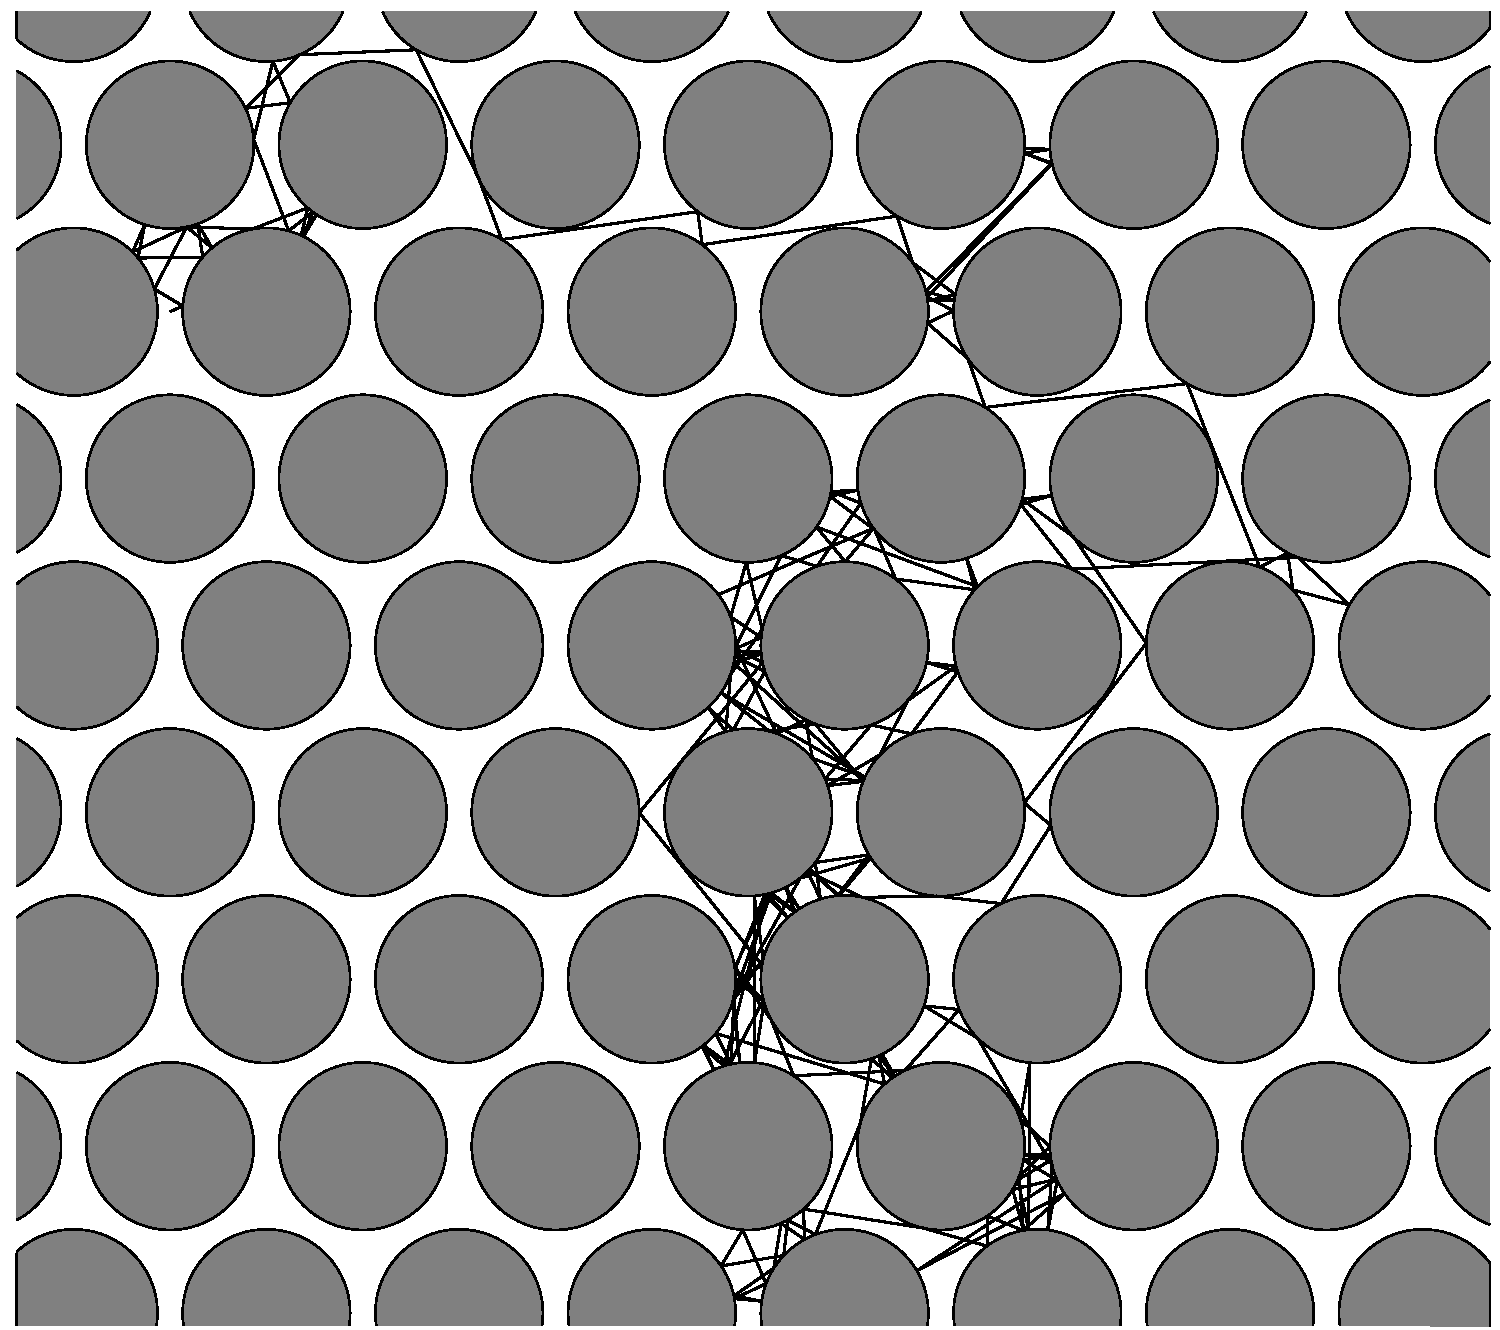
\includegraphics[width=0.45\textwidth]{diffuseChaoticBouncing}
	\end{center}
	\caption[]{\label{fig-chaoticBouncing}
		A chaotic trajectory of a finite horizon Lorentz gas
		point particle bouncing in a
		hexagonal array of disks. The disks are spaced closely enough
		so that the no free flight segment is of infinite length.
	}
\end{figure}

One distinguishes
the {\em infinite horizon} diffusive behavior, which allows for infinite
length flights, from
the {\em finite horizon} case\rf{BunSin81}, where the particle always
hits the next disk in finite time.
Here we shall restrict our consideration to the finite horizon case, with
a triangular tiling of the plane by disks sufficiently large so that no
infinite length free flight is possible. In this case the diffusion is
normal\rf{BunSin81,Bleher92}, with $\timeAver{\hat{x}(t)^2}$ growing like $t$.
% \PC{2015-10-21}{the text from Cvitanovi\'c, Gaspard and Schreiber\rf{CGS92}}
Unfortunately, as we shall see,
the same mechanism that guarantees a finite horizon
also leads to rather awkward grammar rules for admissible itineraries.


The approach introduced in \refref{LorentzDiff} and tested in
\refref{CGS92}, exploits the fact that the periodic Lorentz gas can be
constructed by putting together translated copies of an elementary cell.
Therefore quantities characterizing global dynamics, such as the Lyapunov
exponent and the diffusion constant, can be computed from the dynamics
restricted to the elementary cell.

To investigate the transport properties of such systems, we apply cycle
expansions\rf{DasBuch} to the analysis of {\em diffusion coefficient}.
The resulting formulas are exact; no probabilistic assumptions are made,
and all correlations are taken into account by the  inclusion of cycles
of all periods. While the existing cycle expansion theory\rf{DasBuch} yields the
formally correct
results, the convergence
rate is slow because of bad shadowing and poor choice of symbolic
grammar\rf{CGS92}. In this paper we propose a novel approach that
significantly improves the effectiveness of cycle expansion formulas, by
quotienting the non-commuting rotational and translational symmetries and
using \po s in the fundamental domain (rather than in the elementary cell).


In \refsect{s-Lorentz} we define periodic Lorentz gas, and describe the
symmetry reduction of its full {\statesp} to the elementary
cell and the fundamental domain.

In \refsect{s-elemCell} we describe the elementary cell symbolic dynamics,
and in
\refsect{s-fundDom} we describe the fundamental domain symbolic dynamics.




In \refsect{s-POT}
we briefly review the formulas for diffusion
coefficients in the $2$\dmn\ periodic Lorentz gas, using dynamics
restricted in elementary cell.

In \refsect{s-fundDiff} we
factorize the rotational symmetry and derive the diffusion coefficient
using fundamental domain cycles.

    \PC{2016-07-23} {
reuse this:

The exact results are sometimes counterintuitive, and might help us
decide whether a diffusive phenomenon whose microscopic dynamics is hard
to observe directly, such as conductance fluctuations in a mesoscopic
device, is due to impurities or to deterministic transport. For example,
as some parameter (such as mean free flight time) is increased, the
deterministic diffusion coefficient reveals a non-monotone, fractal
dependence\rf{KlaDor95,KlaDor99,KRS08,KlaKelHow08,DasBuch}.
    }
